\section{Evaluation}
\label{sec:evaluation}

In this section, we quantify the benefits of using a wireless mesh in crowd-shared home networks for public Internet access. In Section \ref{evaluation:environment}, we present the simulation environment, the modeling of router on/off periods, and the metrics used to evaluate the efficiency of the wireless mesh. Section \ref{evaluation:results} provides a comparative study of crowd-shared home networks with and without a wireless mesh based on our simulation results.

\subsection{Simulation Environment}
\label{evaluation:environment}

%Using python, we developed a discrete event simulator to model the behavior of guest flows in a crowd-shared network connected through a wireless mesh network. We use the TFA wireless mesh topology \cite{}, that consist of 21 nodes to model a network of access home routers. Each router possesses an Internet connection from which it provides potential guests with a maximum of 8 Mbps in upload direction. In addition, the nodes are interconnected using an 802.11ac wireless mesh network with a capacity of 200 Mbps.

We developed a simulator that models the behaviour of guests users flows in a crowd-shared WMN. The simulator uses TFA wireless mesh topology [] which consists of 21 nodes (fig. \ref{fig:topology}). Each node in this figure represents a home router with shared internet access bandwidth, whereas each edge is a wireless mesh link. The simulator randomly generates guest users flows at different home routers. Each generated flow has a rate and lifetime sampled out of a uniform and an exponential distribution, respectively. The guests flows arrive to the network according to Poisson process. 

We model the availability of the home access routers using an on-off Markov chain. On and off times are exponentially distributed with mean values $\mu_{on = 106}$ min and $\mu_{off} = 555$ min. We parameterize the exponential distributions using real world data collected from a wireless mesh network in the UK. Figure \ref{fig:active_routers} shows the number of active routers along 60-hours of simulation. We can see that out of 21 routers less than 12 routers are simultaneously available. 

%To reflect real world traffic, we consider guest flows that arrive to the network according to a Poisson process. Each flow has a constant bit rate which is sampled out of a uniform distribution.

\begin{figure}[t]
\begin{center}
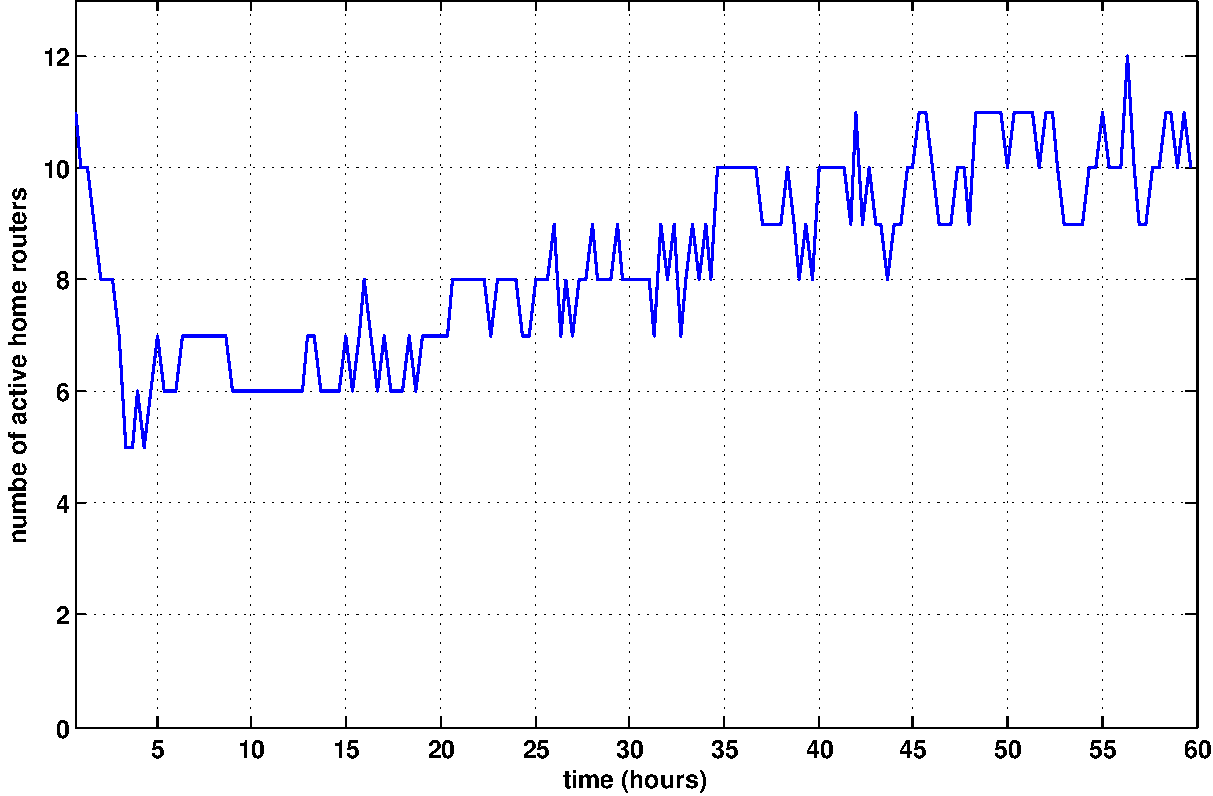
\includegraphics[width=1\linewidth]{results/on_routers.pdf}
\caption{Number of active home routers.}
\label{fig:active_routers}
\end{center}
\end{figure}

%To grant Internet access to the flows, the simulator implements two methods. The first method only give access to flows through the router at which they arrive given that there is enough internet access capacity. This method ignores the mesh network. On the other hand, the second method considers the mesh network by redirecting flows which does not fit in the local access routers to other routers through the mesh network. The router to which the flow is redirected are selected using worst-fit decreasing algorithm. The algorithm starts by sorting the flows to be redirected in non-decreasing order of their rates. Then, for each flow (starting with the flow with the highest rate), the algorithm selects the router with the highest available internet access capacity which fits the flow rate. The shortest path between the router is chosen based on the number of hops. The worst-fit decreasing algorithm is also used to redirect flows when a router goes OFF. This sustains as much as possible flows in the network and reduce disruption by the routers owners sharing policy.
%Furthermore, to show performance of the system under dynamic communication pattern, we consider flows with limited life time which arrive and leave the system at certain time point.

\begin{figure}[t]
\begin{center}
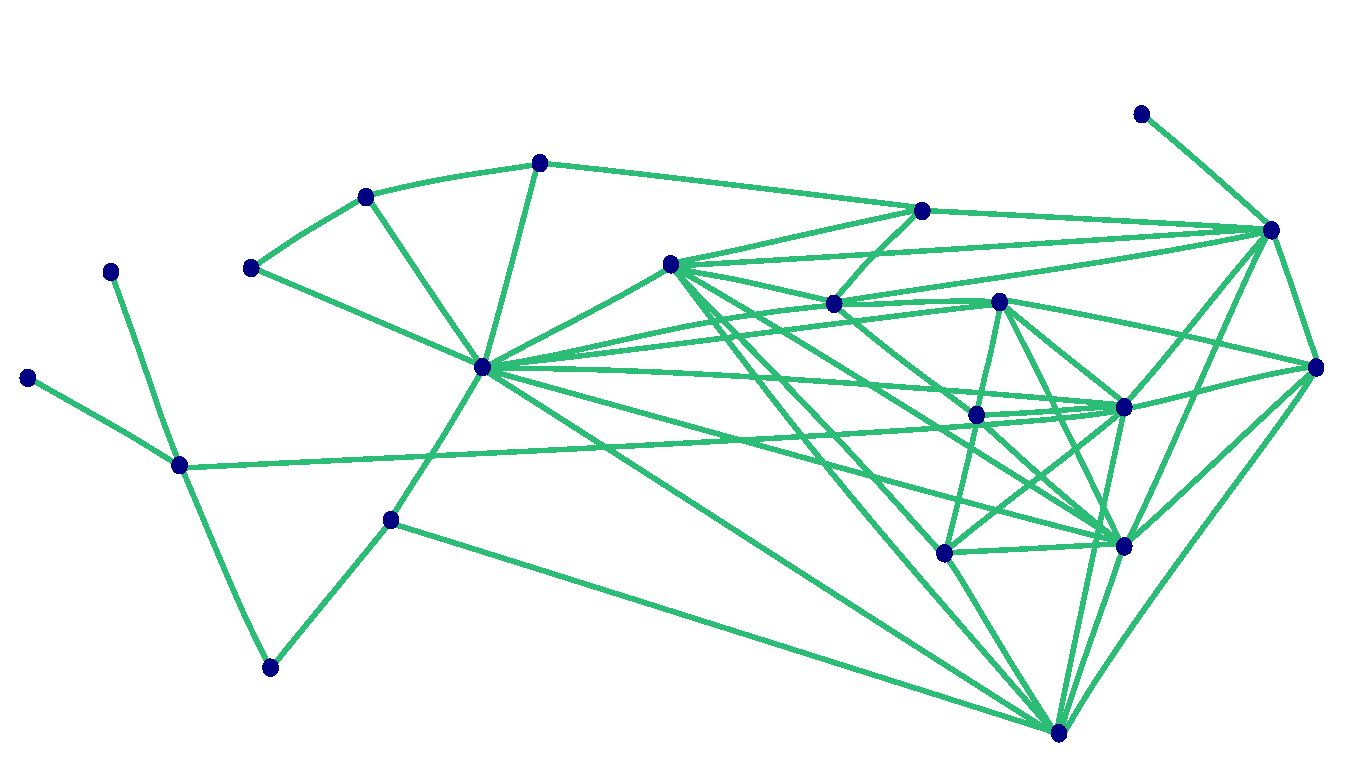
\includegraphics[width=1\linewidth]{topology.pdf}
\caption{Simulation WMN topology.}
\label{fig:topology}
\end{center}
\end{figure}

The simulation proceeds in discrete time ticks. At each time tick, the simulator updates the ON/OFF time of each router, removes expired flows and generates new flows if required. Furthermore, the simulator assign each new flow internet access (a gateway) through their local routers or redirect them to a remote routers based on the algorithm explained in section II-B. The redirection also takes place when routers go off. For each assigned or redirected flow, the simulator updates the available bandwidth of the corresponding router and mesh links.

We compare between crowd-shared home with WMN and without WMN. For each case, we measure the shared bandwidth utilization of the access router as well as the accumulated acceptance rate at each time tick. We define the accumulated acceptance rate $ACR(T)$ at time tick $T$ as :
\vspace{-3mm}
\begin{equation}\label{1}
ACR(T)= \frac{\Sigma^T_t R^{finished}_{t}}{(\Sigma^T_t R^{finished}_{t} + \Sigma^T_t R^{rejected}_{t})}
\end{equation}
\vspace{-2mm}

%${the accumulated acceptance rate =\displaystyle \frac{the\ total\ rates\ of\ flows\ finished\ up\ to\ t} {(the total rates of flows finished up to t + total rates of rejected flows up to t)}}$. 
$R^{finished}_{t}$ denotes the total rates of the flows at time $t$ which are accepted (assigned internet access) and finished successfully without disruption due to router unavailability. $R^{rejected}_{t}$ denotes the total rates of the flows at time $t$ which are rejected (did assigned internet access). 

Due to the large mean values of the ON and OFF times (8 hours OFF and 1.5 hours ON), we run each simulation for 60 hours with time scale of 20 minutes. We perform 20 runs and report the average. We set the shared bandwidth per router to 8 Mbps assuming that each router has a 16 Mbps ADSL access link. We run our simulation with mesh link capacity of 200, 54 and 10 Mbps, however, our results did not show significant difference. 

\subsection{Simulation Results}
\label{evaluation:results}

Initially, we measure the shared bandwidth utilization and request acceptance rate with an arrival rate of 50 flows per minute over a 60-hour period. Fig. \ref{fig:utilization} illustrates a low utilization of the shared bandwidth without a wireles mesh during the whole period, although there is high demand for Internet access by guest users attached to the various home networks. In contrast, a wireless mesh allows to capitilize the unused capacity and accommodate a larger volume of guest user traffic. More precisely, according to Fig. \ref{fig:utilization} guest user traffic redirection through the wireless mesh results in the full utilization of the bandwidth shared by home network users. Furthermore, crowd-shared home networks with a wireless mesh can accommodate substantially higher guest user traffic, as depicted in Fig. \ref{fig:acceptance}. This stems from the high utilization of the shared bandwidth.

\begin{figure}[t]
\begin{center}
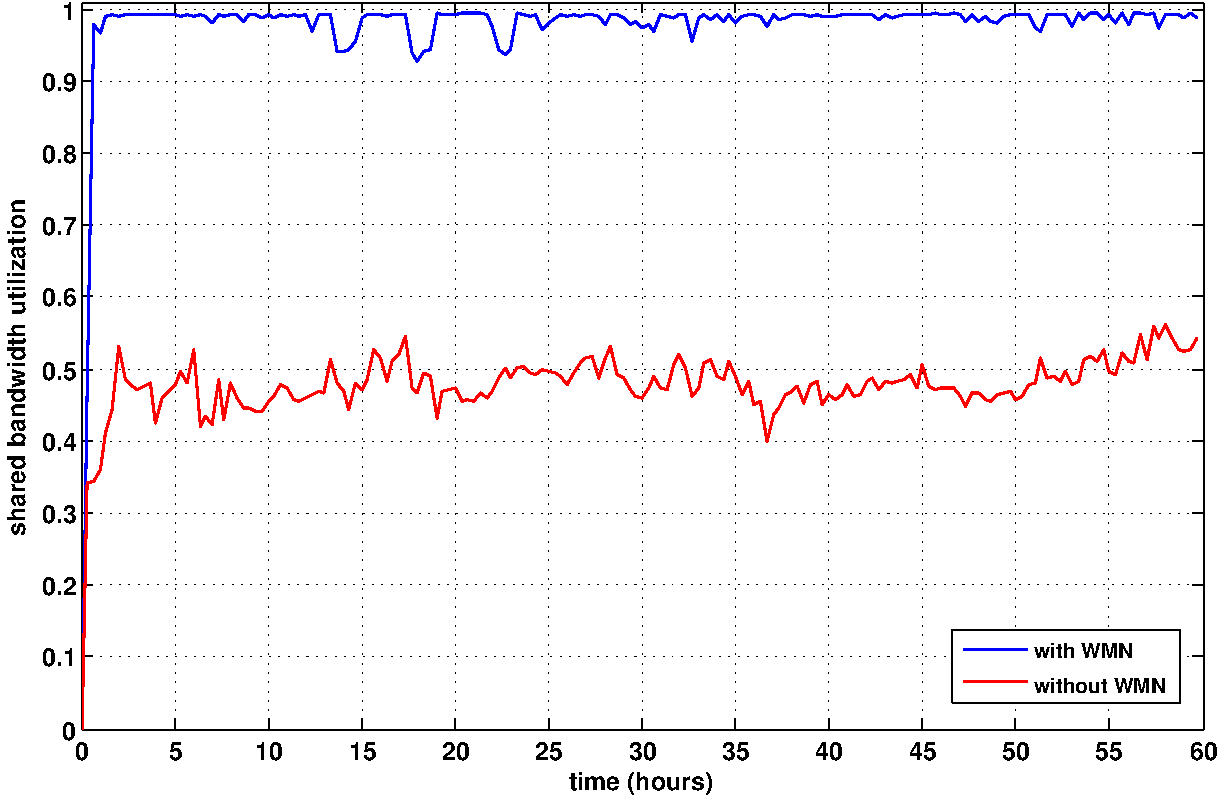
\includegraphics[width=1\linewidth]{results/utilization.pdf}
\caption{Shared bandwidth utilization.}
\label{fig:utilization}
\end{center}
\end{figure}

\begin{figure}[t]
\begin{center}
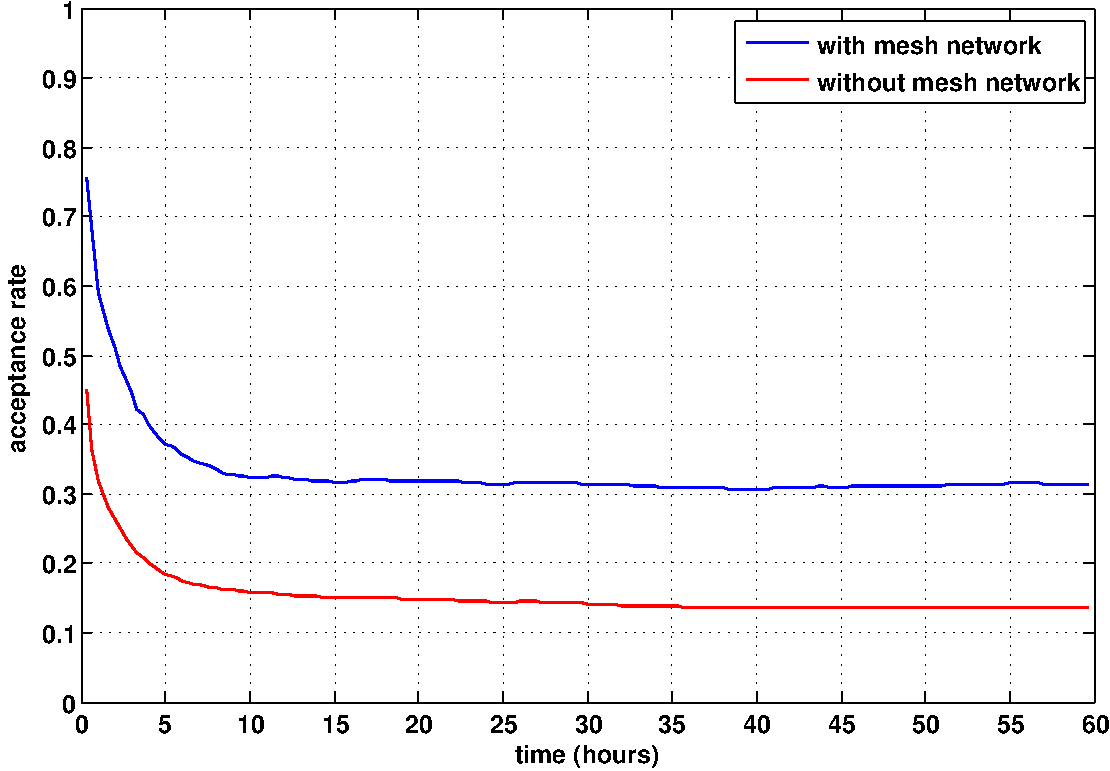
\includegraphics[width=1\linewidth]{results/acceptance_rate.pdf}
\caption{Guest user traffic acceptance rate.}
\label{fig:acceptance}
\end{center}
\end{figure}

We further measure the shared bandwidth utilization with a wide range of guest user traffic demands. In this respect, Fig. \ref{fig:acceptance} illustrates the shared bandwidth utilization with diverse flow arrival rates, ranging from 10 to 100 flows per minute. This simulation result corroborates the efficiency of the wireless mesh for various traffic loads, as the shared bandwidth utilization always remains very high. Without the presence of a wireless mesh, Fig. \ref{fig:utilization_arrival} shows poor bandwidth utilization, especially with low guest user traffic demand. In this particular case, the inability to redirect guest user traffic to home networks with available bandwidth results in wasting most of the shared bandwidth. Eventually, our simulation results show the significant benefit that a wireless mesh can bring in crowd-shared home networks, by effectively pooling shared resources across the interconnected home networks.

\begin{figure}[t]
\begin{center}
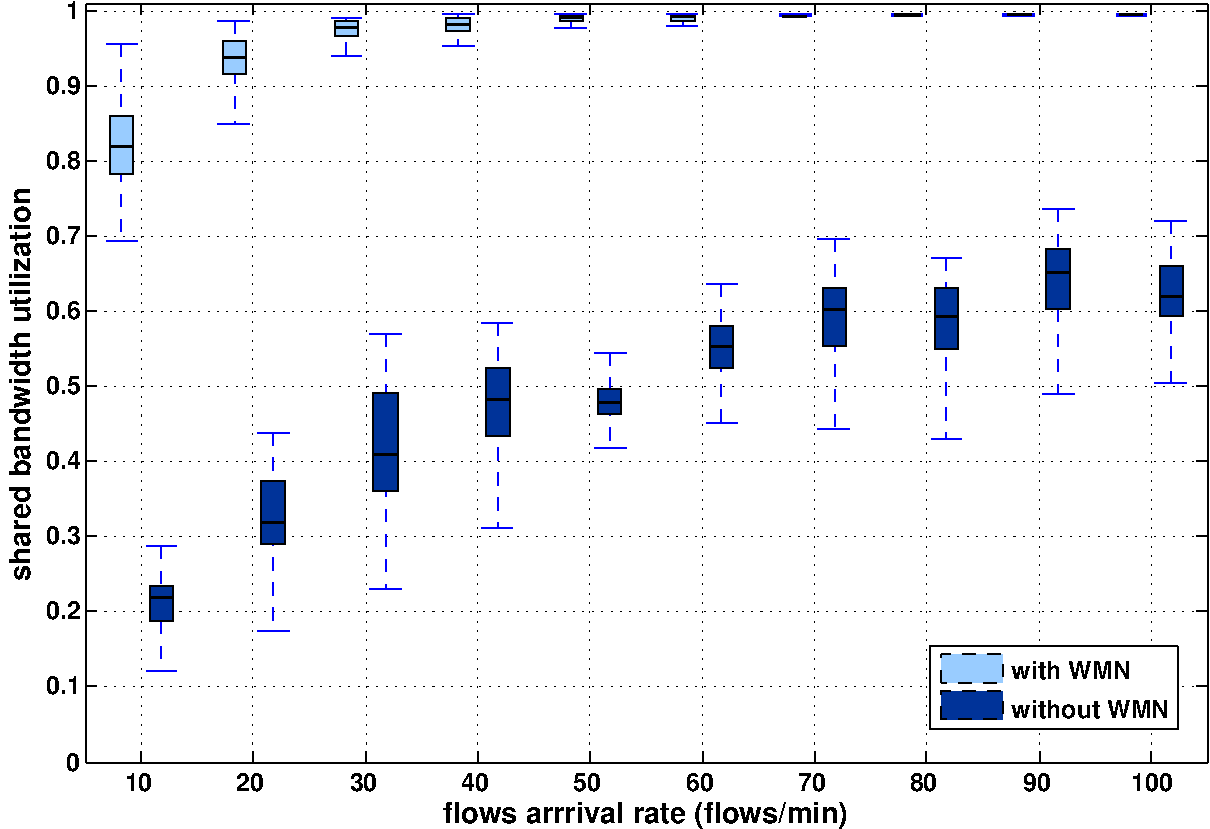
\includegraphics[width=1\linewidth]{results/boxplot2.pdf}
\caption{Shared bandwidth utilization vs. flow arrival rate.}
\label{fig:utilization_arrival}
\end{center}
\end{figure}

According to our simulations, redirected guest user traffic traverses up to 4 hops across the wireless mesh, depending on the home router that has been selected as the Internet gateway. Since this may introduce additional delay and possible variation of delay which may be perceptible by guest users, we measure the shared bandwidth utilization while restricting the number of hops that guest user traffic can traverse. In this respect, Fig. \ref{fig:hop_count} illustrates the shared bandwidth utilization for diverse hop-count thresholds ranging from 1 to 3, and without any limit in the hop count. Restricting the number of hops has a noticeable impact on bandwidth utilization, especially for a single hop, since Internet access is permitted only through one of the next-hop home routers. In essence, there is a trade-off between coverage extension (and thus effective bandwidth utilization) and latency. This may become more critical in large wireless mesh networks, where multi-hop wireless links can inflate latency.


\begin{figure}[t]
\begin{center}
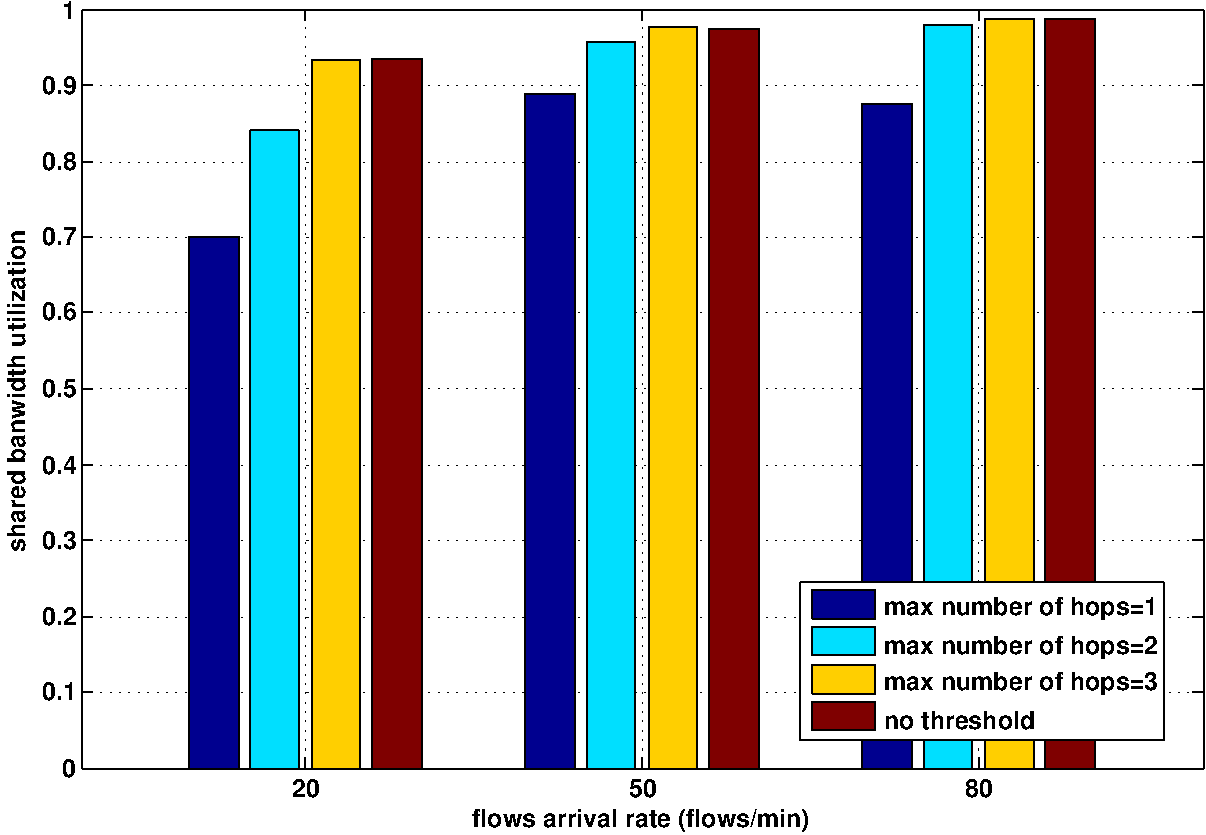
\includegraphics[width=1\linewidth]{results/hops_vs_BW.pdf}
\caption{Shared bandwidth utilization for diverse hop-count threshold values vs. flow arrival rate.}
\label{fig:hop_count}
\end{center}
\end{figure}

